\section{Mechanizmy komunikacji w systemie QNX Neutrino - komunikaty}

\subsection{Wprowadzenie}

W systemie QNX Neutrino istnieje wiele różnych metod komunikacji międzyprocesorowej. Przesyłanie komunikatów (message passing) jest podstawową formą IPC (interprocess communication) w systemie QNX. Ten unikalny dla Neutrino mechanizm został zaimplementowany wprost w mikrojądrze systemu operacyjnego i stanowi prymityw do komunikacji dwukierunkowej modułów (np. menadżera procesów, modułu systemu plików) z mikrojądrem. Pozwala to na odseparowanie procesów od mikrojądra. W przypadku awarii oprogramowania, procesy modułów nie mają bezpośredniego wpływu na działanie mikrojądra. Taka architektura (patrz rysunek~\ref{fig:microkernel}) zapewnia wysoką wydajność, konfigurowalność i skalowalność systemu, dostosowaną do ograniczeń nakładanych na system. Inne mechanizmy IPC (np. omawiane wcześniej potoki i~pliki FIFO) są nadbudową tej formy komunikacji międzyprocesorowej. 


\begin{figure}[!h]
\centering
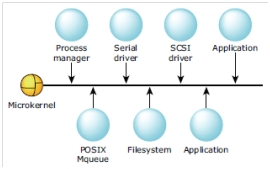
\includegraphics[width=0.5\textwidth]{img/microkernel}
\caption{Modularna architektura QNX Neutrino}
\label{fig:microkernel}
\end{figure}

W zastosowaniach, często spotyka się aplikacje oparte o model klient-serwer, jak na rysunku\ref{fig:clientserver}
. Początkowo serwer czeka na wiadomości od procesów-klientów. Procesy klienta wysyłają (1) dane do serwera, a następnie zostają zablokowane w oczekiwaniu na odpowiedź. W tym czasie serwer otrzymuje wiadomości (2), przetwarza je i odpowiada klientom (3), które kontynuują swoje działanie.

\begin{figure}[!h]
\centering
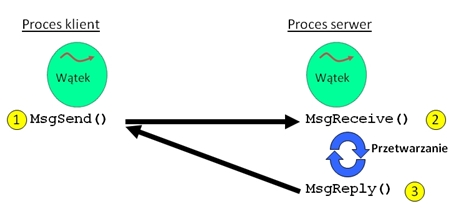
\includegraphics[width=0.65\textwidth]{img/clientserver}
\caption{Model aplikacji typu klient-serwer}
\label{fig:clientserver}
\end{figure}

Ten model wymiany informacji może być zrealizowany poprzez przesyłanie komunikatów (message passing), na który składają się następujące mechanizmy: 

\begin{myitemize}
\item Tworzenie kanałów i połączeń.
\item Wysyłanie, odbieranie i potwierdzanie komunikatów.
\item Impulsy (krótkie, nieblokujące nadawcy komunikaty).
\item Przesyłanie komunikatów poprzez sieć oraz rejestrowanie nazw procesów, w ramach usługi GNS. 
\end{myitemize} 


\subsection{Tworzenie kanałów i połączeń}

W systemie QNX Neutrino przesyłanie komunikatów nie następuje bezpośrednio pomiędzy procesami, czy wątkami. Medium pośredniczącym w przekazywaniu komunikatów jest kanał komunikacyjny. Sytuację pokazano na rysunku~\ref{fig:channels}. Proces serwer, który odbiera komunikaty, tworzy kanał i oczekuje w nim wiadomości od klientów. Procesy klient dołącza się do kanału poprzez połączenia i przez nie wysyła do serwera komunikaty. Klient może mieć wiele połączeń, do różnych serwerów, natomiast serwer używa wyłącznie jednego kanału komunikacyjnego do odbierania wiadomości od klientów. 


\begin{figure}[!h]
\centering
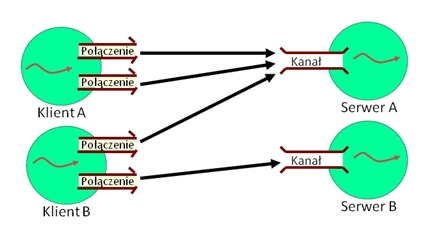
\includegraphics[width=0.65\textwidth]{img/channels}
\caption{Kanały i połączenia}
\label{fig:channels}
\end{figure}

Funkcje służące obsłudze kanałów i połączeń przedstawiono w tabeli~\ref{tab:channels}. 

\begin{table}[h!]
\centering
\caption{Obsługa kanałów i połączeń}
\setlength{\arrayrulewidth}{1pt}
\setlength{\tabcolsep}{6pt}
\renewcommand{\arraystretch}{1.2}
\begin{tabular}{ |p{0.25\textwidth}|p{0.5\textwidth}|}
\hline \rowcolor{gray}
\textbf{Funkcja} & \textbf{Opis} \\ \hline
\mbox{\lstinline[style=MyCStyle]{ChannelCreate()}} & Tworzenie kanału do odbioru wiadomości \\ \hline
\mbox{\lstinline[style=MyCStyle]{ChannelDestroy()}} & Kasowanie kanału \\ \hline
\mbox{\lstinline[style=MyCStyle]{ChannelAttach()}} & Tworzenie połączenia do wysyłania wiadomości \\ \hline
\mbox{\lstinline[style=MyCStyle]{ChannelDetach()}} & Kasowanie połączenia \\ \hline
\end{tabular}
\label{tab:channels}
\end{table}

Pierwszą czynnością, którą należy wykonać przy implementacji serwera jest utworzenie kanału komunikacyjnego. Kanał komunikacyjny jest własnością procesu, który go utworzył. Wątki, które chcą się skomunikować z danym kanałem mogą być zawarte w tym samym procesie, mogą należeć do innego procesu w obrębie tego samego węzła, bądź innego węzła w sieci. Każdorazowo jednak muszą one utworzyć z kanałem połączenie. Kanał komunikacyjny tworzymy za pomocą funkcji:

\begin{lstlisting}[style=MyCStyle]
#include <sys/neutrino.h>
int ChannelCreate( unsigned flags );
int ChannelCreate_r( unsigned flags );
\end{lstlisting}

gdzie \lstinline[style=MyCStyle]{flags} stanowią opcje, które mogą być używane do zmiany własności kanału (tabela~\ref{tab:flags}). 

\begin{table}[h!]
\centering
\caption{Opcje tworzenia kanałów}
\setlength{\arrayrulewidth}{1pt}
\setlength{\tabcolsep}{6pt}
\renewcommand{\arraystretch}{1.2}
\begin{tabular}{ |p{0.3\textwidth}|p{0.5\textwidth}|}
\hline \rowcolor{gray}
\textbf{Opcje} & \textbf{Opis} \\ \hline
\mbox{\lstinline[style=MyCStyle]{_NTO_CHF_COID_DISCONNECT}} & Dostarcz impuls, kiedy dowolne połączenie do kanału jest zamykane. \\ \hline
\mbox{\lstinline[style=MyCStyle]{_NTO_CHF_DISCONNECT}} & Dostarcz impuls, kiedy wszystkie połączenia do kanału są zamknięte.  \\ \hline
\mbox{\lstinline[style=MyCStyle]{_NTO_CHF_FIXED_PRIORITY}} & Nie stosuje dziedziczenia priorytetów. \\ \hline
\mbox{\lstinline[style=MyCStyle]{_NTO_CHF_NET_MSG}} & Zarezerwowane dla menadżera zasobów (ionet) \\ \hline
\mbox{\lstinline[style=MyCStyle]{_NTO_CHF_REPLY_LEN}} & Długość odpowiedzi ma być zawarta w strukturze \mbox{\lstinline[style=MyCStyle]{_msg_info}}, którą wypełnia funkcja \mbox{\lstinline[style=MyCStyle]{MsgReceivev()}}. \\ \hline
\mbox{\lstinline[style=MyCStyle]{_NTO_CHF_SENDER_LEN}} & Długość komunikatu ma być zawarta w strukturze \mbox{\lstinline[style=MyCStyle]{_msg_info}}, którą wypełnia funkcja \mbox{\lstinline[style=MyCStyle]{MsgReceivev()}}. \\ \hline
\mbox{\lstinline[style=MyCStyle]{_NTO_CHF_THREAD_DEATH}} & Dostarcz do kanału impuls, gdy zakończy się dowolny wątek posiadający kanał. \\ \hline
\mbox{\lstinline[style=MyCStyle]{_NTO_CHF_UNBLOCK}} & Dostarcz do kanału impuls, gdy wątek wysyłający będący w stanie \mbox{\lstinline[style=MyCStyle]{REPLY_BLOCKED}} odblokuje się przed wysłaniem mu odpowiedzi funkcją \mbox{\lstinline[style=MyCStyle]{MsgReply()}}.  \\ \hline
\end{tabular}
\label{tab:flags}
\end{table}

Funkcje \lstinline[style=MyCStyle]{ChannelCreate()} i \lstinline[style=MyCStyle]{ChannelCreate_r()}  tworzą kanał komunikacyjny, który może być użyty do odbierania komunikatów lub impulsów. Zwracają identyfikator kanału \lstinline[style=MyCStyle]{CHID} (channel ID) lub \lstinline[style=MyCStyle]{-1} i ustawiają kod błędu. Komunikaty i impulsy są odbierane w kanale komunikacyjnym i ustawiane w kolejkę, zgodnie z wartościami priorytetów. Domyślnie, kiedy proces (wątek) odbiera komunikat z kanału, jego priorytet jest ustawiany w ten sposób, aby był równy priorytetowi procesu (wątku) wysyłającego komunikat. Metoda ta, zwana dziedziczeniem priorytetów (priority inheritance) zapobiega inwersji priorytów. Po otrzymaniu komunikatu, wątek może odłączyć się od kanału poprzez wywołanie \lstinline[style=MyCStyle]{MsgReceive()} z kanału \lstinline[style=MyCStyle]{-1}.  Dziedziczenie priorytetów można wyłączyć, poprzez ustawienie flagi \lstinline[style=MyCStyle]{_NTO_CHF_FIXED_PRIORITY}. Różnica między funkcjami \lstinline[style=MyCStyle]{ChannelCreate()}  i \lstinline[style=MyCStyle]{ChannelCreate_r()} polega na tym, że pierwsza z nich ustawia globalną zmienną \lstinline[style=MyCStyle]{errno}, umożliwiającą odczytanie kodu błędu, a także samego opisu błędu przez funkcję  \lstinline[style=MyCStyle]{char* strerror( int errno );}. 

Aby skasować kanał należy wywołać funkcję:

\begin{lstlisting}[style=MyCStyle]
#include <sys/neutrino.h>
int ChannelDestroy( int chid );
int ChannelDestroy_r( int chid );
\end{lstlisting}


gdzie \lstinline[style=MyCStyle]{chid} - jest numerem kanału zwróconym przez funkcję  \lstinline[style=MyCStyle]{ChannelCreate()}, bądź  \lstinline[style=MyCStyle]{ChannelCreate_r()}.
 
Kiedy kanał jest kasowany, to wszystkie wątki, które są w stanie zablokowany na operacjach  \lstinline[style=MyCStyle]{MsgSend()} i~ \lstinline[style=MyCStyle]{MsgReceive()} zostaną odblokowane. Odbieranie wiadomości, bądź impulsów z kanałów po jego zamknięciu zakończy się niepowodzeniem. 

\begin{example}{[Utworzenie kanału komunikacyjnego]} Skompilować, zbudować oraz uruchomić przykład. 
\lstinputlisting[caption=Kanał komunikacyjny,style=MyCStyle,label=src:channel]{src/lab8/channel.c}
\end{example} 

Ustanowienie połączenia między procesem (wątkiem), a~kanałem wymaga wyłania funkcji \lstinline[style=MyCStyle]{ConnectAttach()}: 

 
\begin{lstlisting}[style=MyCStyle]
#include <sys/neutrino.h>
int ConnectAttach( uint32_t nd,
                   pid_t pid,
                   int chid,
                   unsigned index,
                   int flags );

int ConnectAttach_r( uint32_t nd,
                     pid_t pid,
                     int chid,
                     unsigned index,
                     int flags );
\end{lstlisting}

gdzie 

\begin{myitemize}
\item[] \lstinline[style=MyCStyle]{nd} - jest numerem węzła, na którym uruchomiony jest proces posiadający kanał lub \lstinline[style=MyCStyle]{0}, bądź \lstinline[style=MyCStyle]{ND_LOCAL_NODE}~, w~przypadku węzła bieżącego.
\item[] \lstinline[style=MyCStyle]{pid} - numer PID procesu serwera, tzn. zawierającego kanał komunikacyjny.
\item[] \lstinline[style=MyCStyle]{chid} - jest numerem kanału zwróconym przez funkcję \lstinline[style=MyCStyle]{ChannelCreate()}.
\item[] \lstinline[style=MyCStyle]{index} - najmniejszy akceptowalny numer połączenia; przekazanie flagi \lstinline[style=MyCStyle]{_NTO_SIDE_CHANNEL} powoduje wybranie numeru połączenia z innego zakresu, niż deskryptory plików. Rekomenduje się używanie tej flagi podczas wywołania funkcji. 
\item[] \lstinline[style=MyCStyle]{flags} - flagi modyfikujące działanie; jeśli zawierają \lstinline[style=MyCStyle]{_NTO_COF_CLOEXEC}, to połączenie jest zamykane, kiedy proces wywołuje funkcję z rodziny \lstinline[style=MyCStyle]{exec()}. 
\end{myitemize}

Funkcja zwraca identyfikator połączenia \lstinline[style=MyCStyle]{COID} (connection \lstinline[style=MyCStyle]{ID}), bądź \lstinline[style=MyCStyle]{-1} w przypadku niepowodzenia. Podobnie, jak poprzednio, funkcje \lstinline[style=MyCStyle]{ConnectAttach()} i \lstinline[style=MyCStyle]{ConnectAttach_r()} różnią się ustawianiem zmiennej globalnej \lstinline[style=MyCStyle]{errno}.
 
Zamykanie połączenia realizujemy funkcjami: 

\begin{lstlisting}[style=MyCStyle]
#include <sys/neutrino.h>
int ConnectDetach( int coid );
int ConnectDetach_r( int coid );
\end{lstlisting}

gdzie 

\begin{myitemize}
\item[] \lstinline[style=MyCStyle]{coid} - jest numerem kanału, który chcemy skasować. 
\end{myitemize} 

Funkcja zwraca wartość dodatnią, w przypadku sukcesu i \lstinline[style=MyCStyle]{-1}, w przypadku niepowodzenia. W przypadku wywołanai funkcji, wątki, które są zablokowane na połączeniu, zostaną odblokowane, a funkcja \lstinline[style=MyCStyle]{MsgSend()} zwróci kod błędu. 

\begin{example}{[Utworzenie połączenia]} Skompilować, zbudować oraz uruchomić przykład. Dlaczego wynikiem działania programu jest błąd?
\lstinputlisting[caption=Połączenie,style=MyCStyle,label=src:connect]{src/lab8/connect.c}
\end{example} 

\subsection{Wysyłanie, odbieranie i odpowiadanie na komunikaty}

Komunikacja pomiędzy klientem a serwerem za pomocą przesyłania komunikatów (spotkań) jest komunikacją dwukierunkową, synchroniczną i składa się z trzech etapów: wysyłanie komunikatu przez klienta do serwera, odbiór komunikatu przez serwer i przesłanie przez serwer odpowiedzi do klienta. System operacyjny QNX Neutrino dostarcza całej grupy funkcji, służących do obsługi opisanych trzech etapów komunikacji. Można jednak napisać w pełni funkcjonalne aplikacje typu klient-serwer posługując się minimalnym zestawem funkcji takich, jak: \lstinline[style=MyCStyle]{ChannelCreate()}, \lstinline[style=MyCStyle]{ChannelDestroy()}, \lstinline[style=MyCStyle]{ConnectAttach()}, \lstinline[style=MyCStyle]{ConnectDetach()}, \lstinline[style=MyCStyle]{MsgReply()}, \lstinline[style=MyCStyle]{MsgSend()}, \lstinline[style=MyCStyle]{MsgReceive()}. 

W trakcie komunikacji za pomocą przesyłania komunikatów mogą się zdarzyć dwa scenariusze: 

\begin{myenumerate} 
\item Wywołanie funkcji \lstinline[style=MyCStyle]{MsgSend()} następuje po wywołaniu funkcji \lstinline[style=MyCStyle]{MsgReceive()}. Serwer jest blokowany do momentu nadejścia od nadawcy wiadomości i pozostaje w stanie \lstinline[style=MyCStyle]{RECEIVE blocked} do momentu odebrania wiadomości wysłanej przez klienta. W trakcie przetwarzania danych przez serwer, klient pozostaje w stanie \lstinline[style=MyCStyle]{REPLY blocked}, aż do czasu, gdy otrzyma odpowiedź od serwera. Poza omówionymi stanami, procesy klienta i serwera pozostają w stanie \lstinline[style=MyCStyle]{READY}. Sytuację tę ilustruje rysunek~\ref{fig:Msg1}. 

\begin{figure}[!h]
\centering
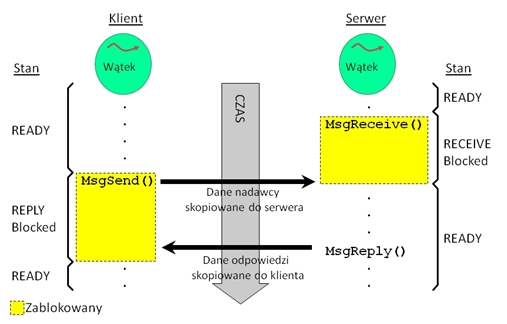
\includegraphics[width=0.75\textwidth]{img/Msg1}
\caption{Ilustracja przesyłania komunikatów - przypadek 1}
\label{fig:Msg1}
\end{figure}

\item Wywołanie funkcji \lstinline[style=MyCStyle]{MsgSend()} następuje przed wywołaniem funkcji \lstinline[style=MyCStyle]{MsgReceive()}. Klient w~stanie \lstinline[style=MyCStyle]{SEND blocked} pozostaje zablokowany  do momentu kiedy serwer rozpocznie odbieranie komunikatu. Jak poprzedni, w trakcie przetwarzania danych przez serwer, klient pozostaje w stanie \lstinline[style=MyCStyle]{REPLY blocked}, aż do czasu, gdy otrzyma odpowiedź od serwera. Poza omówionymi stanami, procesy klienta i serwera pozostają w stanie \lstinline[style=MyCStyle]{READY}. Sytuację tę ilustruje rysunek~\ref{fig:Msg2}. 

\begin{figure}[!h]
\centering
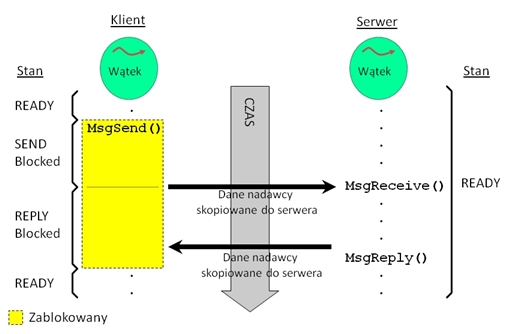
\includegraphics[width=0.75\textwidth]{img/Msg2}
\caption{Ilustracja przesyłania komunikatów - przypadek 2}
\label{fig:Msg2}
\end{figure}
\end{myenumerate} 

Wysyłanie komunikatu realizujemy poprzez następujące wywołanie: 

\begin{lstlisting}[style=MyCStyle]
#include <sys/neutrino.h>

int MsgSend( int coid,
             const void* smsg,
             int sbytes,
             void* rmsg,
             int rbytes );

int MsgSend_r( int coid,
               const void* smsg,
               int sbytes,
               void* rmsg,
               int rbytes );
\end{lstlisting}

gdzie 

\begin{myitemize}
\item[] \lstinline[style=MyCStyle]{coid} - jest numerem kanału, do którego chcemy wysyłać wiadomości. 
\item[] \lstinline[style=MyCStyle]{smsg} - wskaźnik do bufora zawierającego wiadomość do wysłania. 
\item[] \lstinline[style=MyCStyle]{sbytes} - liczba bajtów określająca pojemność bufora do wysłania.
\item[] \lstinline[style=MyCStyle]{rmsg} - wskaźnik do bufora zawierającego odpowiedź. 
\item[] \lstinline[style=MyCStyle]{rbytes} - liczba bajtów określająca pojemność bufora na odpowiedź. 
\end{myitemize}

Funkcja \lstinline[style=MyCStyle]{MsgSend()} wysyła komunikat do kanału określonego przez \lstinline[style=MyCStyle]{coid}. Funkcja ta służy zarówno do wysyłania komunikatu, jak i odbierania wiadomości do serwera. \lstinline[style=MyCStyle]{MsgSend()} zwraca \lstinline[style=MyCStyle]{status}, który jest przekazywany przez \lstinline[style=MyCStyle]{MsgReply()} lub \lstinline[style=MyCStyle]{-1} w przypadku błędu. Działanie funkcji zależy od stanu procesu serwera. Przejścia stanów procesu-klienta zilustrowano na rysunku~\ref{fig:states1}. 

\begin{figure}[!h]
\centering
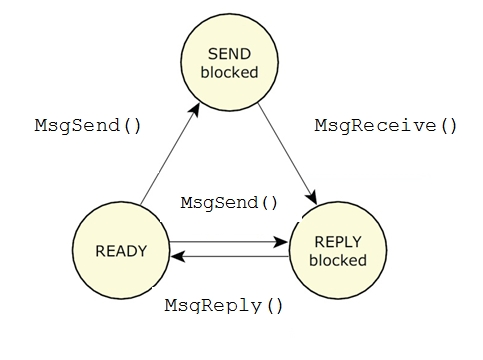
\includegraphics[width=0.5\textwidth]{img/states1}
\caption{Przejścia stanów procesu klienta}
\label{fig:states1}
\end{figure}

Serwer może odebrać komunikat z kanału poprzez wywołanie następującej funkcji: 

\begin{lstlisting}[style=MyCStyle]
#include <sys/neutrino.h>

int MsgReceive( int chid,
                void * msg,
                int bytes,
                struct _msg_info * info );

int MsgReceive_r( int chid,
                  void * msg,
                  int bytes,
                  struct _msg_info * info );
\end{lstlisting}

gdzie

\begin{myitemize}
\item[] \lstinline[style=MyCStyle]{chid} - numer kanału zwrócony przez funkcję \lstinline[style=MyCStyle]{ChannelCreate()}.
\item[] \lstinline[style=MyCStyle]{msg} - wskaźnik do bufora zawierającego odebraną wiadomość. 
\item[] \lstinline[style=MyCStyle]{bytes} - liczba bajtów określająca pojemność bufora do odbioru komunikatu.
\item[] \lstinline[style=MyCStyle]{info} - wskaźnik \lstinline[style=MyCStyle]{NULL}, bądź wskaźnik do struktury \lstinline[style=MyCStyle]{_msg_info}, zawierającej dodatkowe informacje o komunikacie.  
\end{myitemize}

Funkcja odbiera wiadomość, bądź impuls od klienta. W przypadku komunikatu, funkcja zwraca identyfikator nadawcy \lstinline[style=MyCStyle]{rcvid > 0} (receive identifier), w której zakodowano identyfikator wątku (\lstinline[style=MyCStyle]{TID}) wysyłającego i identyfikator połączenia (\lstinline[style=MyCStyle]{COID}). Identyfikator \lstinline[style=MyCStyle]{rcvid} będzie użyty w funkcji \lstinline[style=MyCStyle]{MsgReply()}, wysyłającej do klienta odpowiedź. W przypadku, gdy funkcja odebrała impuls, identyfikator \lstinline[style=MyCStyle]{rcvid = 0}; struktura \lstinline[style=MyCStyle]{_msg_info} nie jest modyfikowana. Przejścia stanów procesu-klienta zilustrowano na rysunku~\ref{fig:states2}

\begin{figure}[!h]
\centering
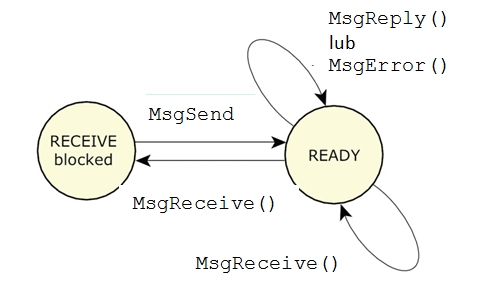
\includegraphics[width=0.5\textwidth]{img/states2}
\caption{Przejścia stanów procesu serwera}
\label{fig:states2}
\end{figure}

Przesłanie odpowiedzi na komunikat można zrealizować funkcją:

\begin{lstlisting}[style=MyCStyle]
#include <sys/neutrino.h>

int MsgReply( int rcvid,
              int status,
              const void* msg,
              int size );

int MsgReply_r( int rcvid,
                int status,
                const void* msg,
                int size );
\end{lstlisting}

gdzie 

\begin{myitemize}
\item[] \lstinline[style=MyCStyle]{rcvid} - identyfikator nadawcy, zwrócony przez funkcję \lstinline[style=MyCStyle]{MsgReceive()}.
\item[] \lstinline[style=MyCStyle]{status} - wartość zwracana przez \lstinline[style=MyCStyle]{MsgSend()}, na której jest zablokowany wątek, którego \lstinline[style=MyCStyle]{ID} jest zakodowane w \lstinline[style=MyCStyle]{rcvid}.  
\item[] \lstinline[style=MyCStyle]{msg} - wskaźnik do bufora zawierającego wysyłaną wiadomość.
\item[] \lstinline[style=MyCStyle]{info} - wskaźnik \lstinline[style=MyCStyle]{NULL}, bądź wskaźnik do struktury \lstinline[style=MyCStyle]{_msg_info}, zawierającej dodatkowe informacje o komunikacie.  
\lstinline[style=MyCStyle]{size} - liczba bajtów określająca pojemność bufora do odpowiedzi.
\end{myitemize}

Funkcja zwraca \lstinline[style=MyCStyle]{0}, gdy wykonała się poprawnie i \lstinline[style=MyCStyle]{-1}, gdy wystąpił błąd. Zanim przejdziemy do napisania prostego szkieletu aplikacji typu klient-serwer spójrzmy na rysunek~\ref{fig:dependencies} prezentujący zależności pomiędzy danymi w procesie Send/Receive/Reply. Oczywiście proces-serwer może odpowiedzieć klientowi, nie wysyłając danych. Scenariusz taki może być użyty w celu odblokowania klienta, kiedy przekazujemy tylko status poprawnego zakończenia do funkcji \lstinline[style=MyCStyle]{MsgSend()}. Realizujemy to przez wywołanie \lstinline[style=MyCStyle]{MsgReply(rcvid, EOK, NULL, 0)}. 

\begin{figure}[!h]
\centering
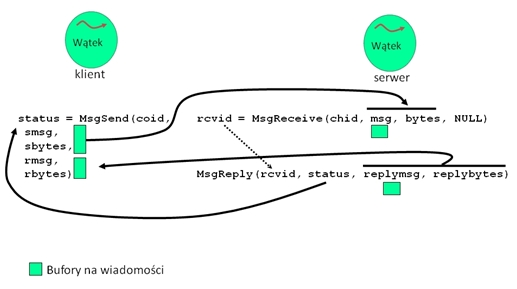
\includegraphics[width=0.75\textwidth]{img/dependencies}
\caption{Zależności pomiędzy danymi w~mechaniźmie komunikatów}
\label{fig:dependencies}
\end{figure}


\begin{example}{[Komunikator typu klient-serwer]} Skompilować oddzielnie program klienta i~program serwera. Najpierw uruchomić serwer, a w~następnej kolejności proces klienta z~odpowiednimi parametrami. 
\lstinputlisting[caption=Szkielet aplikacji typu klient,style=MyCStyle,label=src:client1]{src/lab8/client1.c}
\lstinputlisting[caption=Szkielet aplikacji typu serwer,style=MyCStyle,label=src:server1]{src/lab8/server1.c}
\end{example} 




\subsection{Impulsy}

W aplikacjach często występuje potrzeba powiadomienia procesu o wystąpieniu zdarzenia, ale bez blokady procesu powiadamiającego. System operacyjny QNX Neutrino oprócz synchronicznej komunikacji Send/Receive/Reply, które blokują proces klienta, do czasu, gdy serwer odpowie, wspiera szybką komunikację asynchroniczną. Narzędziem umożliwiającym taką sygnalizację są impulsy (pulses). Impulsy to małe wiadomości, które nie powodują zablokowania procesu wysyłającego. Impuls jest 40-bitowym komunikatem, który zawiera 8-bitowy kod z zakresu od 0 do 127, zdefiniowane w \lstinline[style=MyCStyle]{<sys/neutrino.h>} i~32-bitową wartość, która może być dowolnie wykorzystana przez programistę. Impulsy mogą być odbierane tak, jak inne wiadomości za pomocą funkcji \lstinline[style=MyCStyle]{MsgReceive()}.  Jeśli funkcja odbierze impuls, to zwraca identyfikator nadawcy (receive identifier) równy \lstinline[style=MyCStyle]{0}. We wspomnianym pliku nagłówkowym zdefiniowano impuls, jako następującą strukturę: 

\begin{lstlisting}[style=MyCStyle]
struct _pulse {
_uint16 type;
_uint16 subtype;
_int8 code;
_uint8 zero [3];
union sigval value;
_int32 scoid;
};
union sigval {
int sival_int;
void *sival_ptr;
};
\end{lstlisting}

Najważniejsze pola tej struktury dotyczą elementów code oraz value. Pole code identyfikuje typ impulsu, natomiast element value jest uzupełnieniem pola code i może być dowolnie ustawione, w przeciwieństwie do innych pól tej struktury. 
Impulsy można wysyłać za pomocą funkcji \lstinline[style=MyCStyle]{MsgSendPulse()}: 

\begin{lstlisting}[style=MyCStyle]
#include <sys/neutrino.h>

int MsgSendPulse ( int coid,
                   int priority,
                   int code,
                   int value );
\end{lstlisting}

gdzie

\begin{myitemize}
\item[] \lstinline[style=MyCStyle]{coid} - identyfikator połączenia, ustanowiony przez funkcję \lstinline[style=MyCStyle]{ConnectAttach()}.
\item[] \lstinline[style=MyCStyle]{priority} - priorytet impulsu. 
\item[] \lstinline[style=MyCStyle]{code} - 8-bitowy pole kodu wysyłanego impulsu, określający jego typ. Bezpieczny zakres kodu mieści się między wartością \lstinline[style=MyCStyle]{_PULSE_CODE_MINAVAIL},  a watością  \lstinline[style=MyCStyle]{_PULSE_CODE_MAXAVAIL}.
\item[] \lstinline[style=MyCStyle]{value} - 32-bitowy komunikat.
\end{myitemize}


Funkcja \lstinline[style=MyCStyle]{MsgSendPulse()} umożliwia nieblokujące przekazanie 32-bitowego komunikatu do kanału komunikacyjnego, identyfikowanego przez \lstinline[style=MyCStyle]{coid}. Funkcja zwraca \lstinline[style=MyCStyle]{-1} w przypadku błędu oraz inną wartość, gdy wykona się prawidłowo. Impulsy można odbierać za pomocą funkcji \lstinline[style=MyCStyle]{MsgReceive()}. Jeśli jednak proces ma odbierać tylko impulsy, to można zastosować funkcję \lstinline[style=MyCStyle]{MsgReceivePulse()}.  Opis funkcji można znaleźć w dokumentacji systemu. 

\begin{example}{[Komunikator typu klient-serwer-impulsy]} Skompilować oddzielnie program klienta i~program serwera. Najpierw uruchomić serwer, a w~następnej kolejności proces klienta z~odpowiednimi parametrami. 
\lstinputlisting[caption=Szkielet aplikacji typu klient,style=MyCStyle,label=src:client2]{src/lab8/client2.c}
\lstinputlisting[caption=Szkielet aplikacji typu serwer,style=MyCStyle,label=src:server2]{src/lab8/server2.c}
\end{example} 


\subsection{W jaki sposób klient znajduje serwer?}

Kiedy proces klienta komunikuje się z procesem serwera potrzebuje trzech informacji: identyfikator węzła ND, numer PID procesu serwera oraz identyfikator kanału CHID. W dotychczasowych przykładach, komunikacja występowała na lokalnym węźle, a numery PID i CHID były przekazywane z linii poleceń. W~jaki sposób, w ogólnym przypadku, klient ma uzyskać od serwera informacje o numerach ND/PID/CHID? Istnieje wiele rozwiązań tego problemu. Wybrane sposoby, wg wzrastającego stopnia ogólności podano poniżej.

\begin{myenumerate} 
\item W ustalonym i znanym miejscu serwer tworzy plik tekstowy, w którym będą przechowywane numery ND/PID/CHID. Plik ten może być następnie przeczytany przez procesy klientów. Metoda ta jest często stosowana w systemach UNIX-owych. 
\item Użycie zmiennych globalnych do przechowywania informacji o zmiennych ND/PID/CHID. Sytuacja ta jest typowa dla przypadku procesów macierzystych i potomnych, a także serwerów wielowątkowych.
\item Użycie mechanizmu globalnych nazw GNS (Global Name Service), takich jak \lstinline[style=MyCStyle]{name_attach()}, \lstinline[style=MyCStyle]{name_detach()}, \lstinline[style=MyCStyle]{name_open()} i \lstinline[style=MyCStyle]{name_close()}. 
\item Utworzyć serwer, jako menadżer zasobów. Do identyfikacji procesu serwera można użyć przestrzeni nazw plików. 
\end{myenumerate} 


Pierwsza metoda, pomimo, że dość prosta w implementacji, posiada istotne wady. Utworzone przez serwer pliki z informacjami ND/PID/CHID pozostają w pamięci nawet w przypadku, gdy proces serwera zostanie zakończony, a dane stracą swoją ważność. Może się również zdarzyć sytuacja, że system operacyjny utworzy inny proces o takich samych danych ND/PID/CHID, jak w pliku. W tym przypadku, komunikaty mogą trafić do niewłaściwego adresata i spowodować niepoprawne działanie systemu. 

Drugie podejście wymaga zastosowania zmiennych globalnych do przekazywania informacji o ND/PID/CHID. Rozwiązanie to działa w zakresie pamięci wspólnej, wykluczona jest komunikacja sieciowa. Metoda ta może być stosowana w przypadku aplikacji wieloprocesorowych i wielowątkowych. Proces (wątek) serwera tworzy kanał komunikacyjny i umieszcza w zmiennych globalnych PID/CHID, które następnie mogą być odczytane przez procesy (wątki) klientów. 

Trzecie podejście polega na zastosowaniu mechanizmu globalnych nazw (Global Name Service). Mechanizm ten działa dobrze w przypadku prostych aplikacji typu klient-serwer. 

Ostatnie rozwiązanie jest najbardziej ogólne spośród wymienionych. Proces serwera staje się menadżerem zasobów. Serwer rejestruje unikalną nazwę ścieżki dostępu, natomiast klient może wtedy wykonać prostą operację open() na tej ścieżce. Opis menadżerów zasobów można znaleźć w~dokumentacji QNX. 

\subsection{Ćwiczenia}

\begin{myenumerate}
\item Wywołać w wierszu poleceń funkcję \lstinline[style=MyCStyle]{pidin | more}. Obejrzeć wyniki, zwrócić uwagę na kolumnę STATE i BLOCKED. Pierwsza z nich wskazuje stan procesu. Druga z nich, w przypadku stanu REPLY pokazuje PID procesu serwera, od którego czekamy na odpowiedź, bądź w przypadku stanu RECEIVE pokazuje nr kanału, w którym oczekujemy wiadomości. Otworzyć perspektywę QNX System Information Perspective. Obejrzeć widoki Process Information, Connection Information i~System Blocking Graph. 
\item Na bazie szkieletu aplikacji klient-serwer, napisać program klienta, który będzie w pętli pobierał od użytkownika linie tekstu ze standardowego wejścia (użyć funkcji: \lstinline[style=MyCStyle]{char *fgets(char *str, int size, FILE *stream);} a następnie będzie przekazywał komunikat do serwera. Serwer w~odpowiedzi ma wyświetlać na ekranie komunikat i wysyłać do klienta przerobiony komunikat, opatrzony nagłówkiem (dowolnym napisem, np. ***). Niech informacje o numerach ND/PID/CHID będą przekazywane poprzez plik tekstowy. 
\end{myenumerate} 


\cleardoublepage
